\section{Grader} \label{sec:grader}
Når man arbejder med grafer, kan det være brugbart at vide, hvor mange kanter der er incidente med en knude. Dertil bruger man følgende definition:

%-----------------------------------------------
\begin{defn}[Grader] \label{defn:grader}
Lad $v \in V$ være en vilkårlig knude i den ikke-orienterede graf, $G = (V,E)$. For $G$ skal det gælde, at den enten er simpel eller en multigraf. Knudens \emph{grad}, $\deg(v)$, er det antal kanter i mængden, $E$, som er incidente med $v$. Dermed gælder det, at
\begin{equation}
\deg(v)=|\{ \{u,v\} \ | \ \{u,v\}\in E \}|.
\end{equation}
\end{defn}

Definition \ref{defn:grader} gælder ikke for pseudografer, da den kun vil tælle en løkke, $\{v\}$, en enkelt gang. Dette er et problem, eftersom løkker tæller dobbelt, idet de både starter og slutter i knuden.

\begin{exmp} \label{ex:grader}

Vi kan ud fra Definition \ref{defn:grader} aflæse knudernes grader på \autoref{fig:grader}. Ved at tælle antallet af knudernes incidente kanter får vi: $\deg(v_{1})=3, \ \deg(v_{2})=3, \ \deg(v_{3})=4$ og $\deg(v_{4})=2$.


\begin{figure}[H]
\centering
	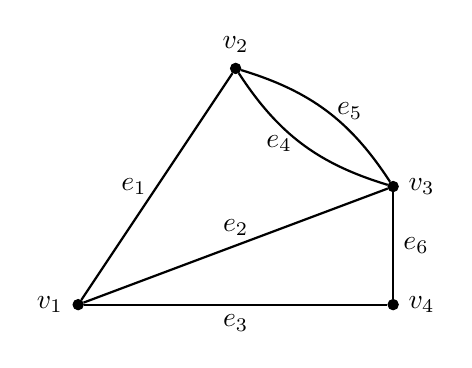
\begin{tikzpicture}[every loop/.style={}]
      \tikzset{enclosed/.style={draw, circle, inner sep=0pt, minimum size=.13cm, fill=black}}
%% Vertices
      	\node[enclosed, label={left: $v_1$}] (v1) at (0,0) {};
      	\node[enclosed, label={above: $v_2$}] (v2) at (2,3) {};
    	\node[enclosed, label={right: $v_3$}] (v3) at (4,1.5) {};
  	    \node[enclosed, label={right: $v_4$}] (v4) at (4,0) {};
%Edges
		\path[thick] (v2) edge [bend right=20] node[midway, left] {$e_4$} (v3);
		\path[thick] (v3) edge [bend right=20] node[midway, right] {$e_5$} (v2);
		\path[thick] (v1) edge node[midway, above] {$e_2$} (v3);
		\path[thick] (v1) edge node[midway, below] {$e_3$} (v4);
		\path[thick] (v1) edge node[midway, left] {$e_1$} (v2);
		\path[thick] (v3) edge node[midway, right] {$e_6$} (v4);
	\end{tikzpicture}
	\caption{Multigraf.}
	\label{fig:grader}
\end{figure}


\end{exmp}

Foruden kanternes grad, kan man også snakke om grafens samlede grad.

\begin{thm}
Hvis en graf, $G = (V,E)$, er en ikke-orienteret, endelig graf med en mængde kanter, $E$, og hvis en knude, $v$, har graden $\deg(v)$, gør det sig gældende, at
\begin{equation} \label{eq:degv=2e}
	\sum_{v \in V} { } \deg(v) = 2 \cdot |E|.
\end{equation}
\end{thm}

Hvis vi har en ikke-orienteret, endelig graf, kan antallet af kanter i grafen findes ved at lægge summen af hver knudes grad sammen og dividere denne sum med to. Omvendt kan grafens samlede grad findes ved at gange antallet af kanter med to.

\begin{proof}
Som det fremgår af Definition \ref{def:graf}, er $E$ en delmængde af mængden, $\{\{u,v\}|u,v \in V \}$. Hver kant i grafen er altså incident med to knuder, eller med den samme knude to gange, hvis der er tale om en løkke. Hvis en kant er incident med en knude, $v$, bidrager denne kant til knudens grad. Hver kant bidrager altså to gange til grafens grad. Hele grafens grad, $\sum_{v \in V} { } \deg(v)$, vil dermed være dobbelt så stor som antallet af kanter i denne graf, $|E|$. 
\begin{equation}
\sum_{v \in V} { } \deg(v) = 2 \cdot |E|.
\end{equation} 
\end{proof}

I en orienteret graf tælles knudernes grader på anden vis. Kanterne har en startknude og en endeknude, og derfor deles graderne i en orienteret graf op i den \emph{indadgående grad} og den \emph{udadgående grad}. 

\begin{defn}[Indadgående grad]
Lad $v \in V$ være en knude i den orienterede graf, $G = (V,E)$. Knudens indadgående grad, $\deg^-(v)$, er det antal kanter i $E$, der har $v$ som endeknude. Dermed gælder det, at
\begin{equation}
\deg^-(v)=|\{(u,v) \ | \ (u,v) \in E \}|.
\end{equation}
\end{defn}

\begin{defn}[Udadgående grad]
Lad $v \in V$ være en knude i den orienterede graf, $G = (V,E)$. Knudens udadgående grad, $\deg^+(v)$, er det antal kanter i $E$, som har $v$ som startknude. Dermed gælder det, at
\begin{equation}
\deg^+(v)=|\{(v,u) \ | \ (v,u) \in E \}|.
\end{equation}
\end{defn}

Vi kan bruge disse to definitioner til at finde graden i en orienteret graf. 

\begin{defn}[Graden i en orienteret graf]
I en orienteret graf, $G = (V,E)$, hvor $v \in V$, er den samlede grad defineret ved: 
\begin{equation}
\sum_{v \in V} { } \deg(v) = \sum_{v \in V} { } \deg^{-}(v) + \sum_{v \in V} { } \deg^{+}(v).
\end{equation}
\end{defn}

Da hver kant skal have en start- og endeknude, må det gælde, at 
\begin{equation}
|E|= \sum_{v \in V} { } \deg^{-}(v) = \sum_{v \in V} { } \deg^{+}(v),
\end{equation}
og derfor må \autoref{eq:degv=2e} også gælde for orienterede grafer.

%
%
%\texttt{%
%
%\begin{defn}[]
%
%og da 
%
%
%
%
%
%vil graden i en orienteret graf, $G = (V,E)$, være 
%


\begin{exmp} \label{ex:grader_orienteret}
Vi kan nu beregne antallet af indadgående og udadgående grader i \autoref{fig:grader_orienteret}.
\input{fig/tikz/grafer/grader_orienteret_eksempel}
Vi ser, at $\deg^{+}(v_{1})=3$, $\deg^{-}(v_{1})=0$, $\deg^{+}(v_{2})=1$, $\deg^{-}(v_{2})=2$, $\deg^{+}(v_{3})=2$, $\deg^{-}(v_{3})=2$, $\deg^{+}(v_{4})=1$ og $\deg^{-}(v_{4})=3$. Vi ser altså, at en løkke tæller som både en indadgående kant og en udadgående kant.
\end{exmp}

